\documentclass{article}
\usepackage{amsmath}
\usepackage{amssymb}
\usepackage{graphicx}
\usepackage{hyperref}
\usepackage[version=4]{mhchem}


\begin{document}
As shown in the figure, two diagonals \(A C\) and \(B D\) of quadrilateral \(A B C D\) intersect at \(O\). Find the length of \(A D\) if \(B O=4\), \(O D=6, A O=8, O C=3\), and \(A B=6\).\\
(A) \(9 \sqrt{7}\)\\
(B) \(8 \sqrt{7}\)\\
(C) \(6 \sqrt{7}\)\\
(D) \(8 \sqrt{2}\) \(\sqrt{166}\)\\
(E)

Solution: (E).\\
\centering
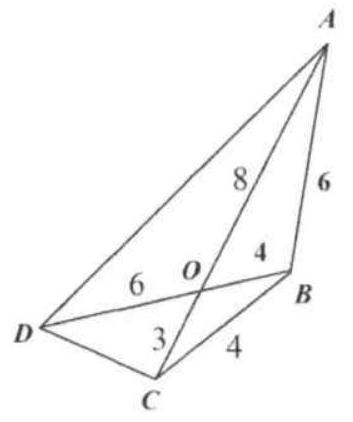
\includegraphics[width=\textwidth]{images/081(2).jpg}


Denote \(F\) as the foot of the perpendicular from \(A\) to an extended diagonal \(D B\), and denote \(B F\) and \(F A\) by \(x\) and \(y\) respectively (see figure). By the Pythagorean Theorem, \(x^{2}+y^{2}=6^{2}\) and \((x+4)^{2}+y^{2}=8^{2}\).\\
Subtracting the first of these equations from the second yields\\
\(8 x+16=28, x=3 / 2\).\\
Substitute the value of x into the first equation and solve for \(y^{2}\) :\\
\centering
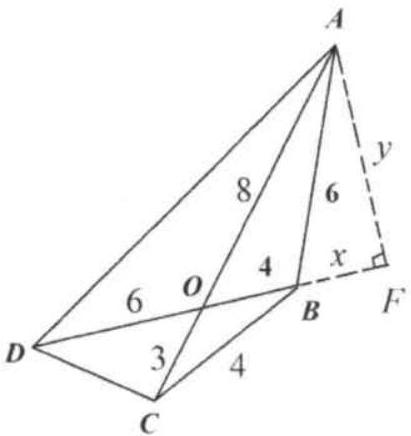
\includegraphics[width=\textwidth]{images/082(2).jpg}\\
\(\left(\frac{3}{2}\right)^{2}+y^{2}=6^{2} \Rightarrow \quad y^{2}=\frac{135}{4}\).\\
Therefore \(A D^{2}=(10+x)^{2}+y^{2}=\left(\frac{23}{2}\right)^{2}+\frac{135}{4}=\frac{664}{4}=166\).\\
\(A D=\sqrt{166}\).


\end{document}
